% !TeX root = er.tex

\chapter{Robotique en essaim}\label{ch.swarm}
\index{robotique en essaim}

Les usines utilisent plusieurs robots pour atteindre des objectifs tels que la peinture et le soudage d'une voiture (\ref{fig.assemblyline}). L'utilisation de plusieurs robots permet de réduire le temps de fabrication en effectuant simultanément différentes tâches telles que le soudage de pièces des deux côtés d'une voiture. Ces tâches sont généralement conçues pour être indépendantes, sans collaboration étroite entre les robots. Plus tard, les robots, en particulier les robots mobiles, ont été conçus pour collaborer les uns avec les autres afin d'effectuer plusieurs actions simultanément à différents endroits.

Voici quelques exemples de tâches nécessitant la collaboration de plusieurs robots :
\begin{itemize}
\item Manipulation de grands éléments structurels dans les bâtiments, ainsi que dans des environnements difficiles d'accès pour les humains, comme dans l'espace ou sous l'eau.
\item Exécuter une tâche grâce à la collaboration de différents types de robots : lors d'une catastrophe de grande ampleur, un drone volant peut localiser les zones où des victimes sont susceptibles d'être trouvées, tandis qu'un robot à chenilles au sol fouille ces zones, en se concentrant sur les endroits qui peuvent être cachés de l'observation aérienne par des arbres ou des décombres.
\item Effectuer des mesures simultanées à différents endroits : mesurer les perturbations sonores dans différentes parties d'un bâtiment, ou surveiller la pollution après un accident industriel. 
\end{itemize}
Le point commun de ces situations est que plusieurs robots participent à l'exécution d'une tâche et qu'ils doivent se coordonner parce qu'ils agissent sur le même objet physique, même s'ils ne sont pas à côté l'un de l'autre dans l'environnement. 

La collaboration entre robots peut également être utilisée pour accélérer l'exécution d'une tâche en demandant à plusieurs robots de l'effectuer en parallèle. Prenons l'exemple de la mesure de la pollution sur une vaste zone : un seul robot peut parcourir toute la zone (comme un aspirateur robotisé dans un appartement), mais la tâche sera accomplie beaucoup plus rapidement si plusieurs robots se répartissent les zones à couvrir.

\section{Approches de la mise en œuvre de la collaboration entre robots}

Il existe deux approches principales de la conception de systèmes composés de plusieurs robots. La première est un \textit{système centralisé}, dans lequel un composant central (l'un des robots ou un ordinateur externe) coordonne tous les robots et leurs tâches. L'avantage d'un système centralisé est qu'il est relativement simple à mettre en œuvre. Son principal inconvénient est qu'il est difficile à étendre, car l'ajout de robots ajoute une charge de traitement à la station centrale où toute l'intelligence est concentrée. Dans un système centralisé, les robots eux-mêmes peuvent être "stupides", mais la plupart des robots ont une puissance de calcul importante qui n'est pas bien utilisée dans cette architecture. Un autre inconvénient majeur d'un système centralisé est que le composant central est un point de défaillance unique. S'il cesse de fonctionner, c'est tout le système qui tombe en panne. Dans les environnements critiques, il est inacceptable d'utiliser un système qui n'est pas robuste en cas de défaillance d'un seul composant.

Si nous nous tournons vers le monde animal, nous constatons que de nombreuses activités sont \emph{distribuées},\index{robotique en essaim!architecture distribuée}, c'est-à-dire que des individus indépendants travaillent ensemble pour atteindre des objectifs communs à l'ensemble de la population. Les fourmis optimisent leur chemin vers les sources de nourriture non pas en dépendant d'une fourmi qui en envoie d'autres à la recherche et qui traite ensuite les informations obtenues, mais par un effort distribué de l'ensemble de la colonie de fourmis. Chaque fourmi marque le sol avec des phéromones qui sont détectées par les autres fourmis. Si quelques fourmis sont dévorées par un prédateur, le reste de la colonie survit, tout comme les connaissances incorporées dans les emplacements des phéromones. L'efficacité et la robustesse de cette approche ont été démontrées dans les algorithmes du chapitre \ref{ch.obstacle}.

\emph{La robotique en essaim} est une approche distribuée de la robotique qui tente de coordonner le comportement en copiant des mécanismes inspirés du comportement des animaux sociaux. Ces mécanismes, souvent locaux et simples, permettent à un groupe d'atteindre des performances globales qui ne pourraient pas être atteintes par un individu seul. Les systèmes distribués présentent les avantages suivants :
\begin{itemize}
\item Ils sont robustes. La perte d'un robot sur dix ne réduit les performances du système que d'environ $10\%$, au lieu d'entraîner la défaillance de l'ensemble du système.
\item Ils sont flexibles et évolutifs. Le nombre de robots peut être adapté à la tâche. S'il y a dix robots dans le système mais que cinq suffisent à accomplir la tâche, les cinq autres peuvent être affectés à d'autres tâches, tandis que si dix robots ne peuvent pas accomplir la tâche efficacement, dix autres peuvent facilement être ajoutés.
\end{itemize}
Ces avantages s'accompagnent d'un effort de conception et de mise en œuvre de la coordination entre les robots. En robotique en essaim, comme dans la nature, il existe des mécanismes de coordination relativement simples qui rendent les systèmes distribués réalisables.

Ce chapitre présente deux approches de la coordination en robotique en essaim : \begin{itemize}
\item Coordination basée sur l'information (Sec.\ref{s.swarm-info}), où l'interaction prend la forme de communications entre les robots. Il peut s'agir d'une communication directe par la transmission explicite de messages électroniques ou d'une communication indirecte par l'insertion de messages dans l'environnement.
\item Coordination physique (Sec.~\ref{s.swarm-physical}), où les robots individuels interagissent au niveau mécanique, soit directement en exerçant des forces les uns sur les autres, soit indirectement en manipulant un objet commun.
\end{itemize}

\section{Coordination par échange local d'informations}\label{s.swarm-info}\index{robotique en essaim!échange d'informations@par échange d'informations}

Les communications peuvent être globales ou locales. Supposons que vous receviez un appel de vos amis et qu'ils vous informent : "Nous voyons un marchand de glaces sur la gauche. Cette information est inutile à moins qu'ils ne vous indiquent leur position actuelle. En revanche, si vous marchez côte à côte avec eux et que l'un d'eux vous dit : "Je vois un magasin de glaces sur la gauche", cette information \emph{locale} vous permet de connaître immédiatement l'emplacement approximatif du magasin et de le localiser facilement visuellement.

Inspirée par la nature, la robotique en essaim utilise des communications locales au sein d'une architecture distribuée. Quelques zèbres situés à la périphérie d'un troupeau recherchent des prédateurs et signalent les autres par des sons ou des mouvements. Le troupeau est une stratégie de survie efficace pour les animaux, car les communications locales permettent à un grand nombre d'animaux de fuir immédiatement lorsqu'un prédateur est détecté par un petit nombre d'observateurs vigilants.

\subsection{Communications directes}
\index{robotique en essaim!communications électroniques@par communications électroniques}

\emph{Direct} L'échange local d'informations est réalisé lorsqu'un ami vous parle. Les animaux ne parlent pas, mais ils utilisent le son ainsi que le mouvement et le contact physique pour réaliser un échange local direct d'informations. Les robots mettent en œuvre des communications locales directes par voie électronique (WiFi ou Bluetooth), ou en transmettant et en recevant de la lumière ou des sons. Ils peuvent également utiliser une caméra pour détecter des changements chez un autre robot, par exemple en allumant une lumière. 

Les communications locales peuvent être soit \emph{directionnelles}, soit \emph{non-directionnelles}. Les communications radio telles que Bluetooth sont locales (quelques mètres seulement) et le robot récepteur ne cherche généralement pas à déterminer la direction du robot émetteur. Les communications directionnelles locales peuvent être mises en œuvre en utilisant une source lumineuse comme émetteur et un détecteur à ouverture étroite ou une caméra comme récepteur.

\subsection{Communications indirectes}
\index{robotique en essaim!communications à l'aide d'objets}

\emph{Les communications locales indirectes} font référence aux communications par l'intermédiaire d'un support qui peut stocker un message transmis en vue d'un accès ultérieur. L'exemple le plus familier est le courrier, qu'il s'agisse de courrier électronique ou de courrier ordinaire, où l'émetteur compose le message et l'envoie, mais où le message reste sur le serveur ou au bureau de poste jusqu'à ce qu'il soit remis au destinataire qui, à son tour, peut ne pas y avoir accès immédiatement. Les communications indirectes chez les animaux sont appelées \emph{stigmergy} ; les animaux laissent des messages en déposant des substances chimiques que d'autres animaux peuvent percevoir. Nous avons mentionné l'utilisation des phéromones par les fourmis ; un autre exemple est l'utilisation de l'urine par un chien pour marquer son territoire.

Les messages chimiques sont difficiles à mettre en œuvre dans les robots, mais les robots peuvent laisser des marques optiques sur le sol, comme nous l'avons fait dans l'algorithme simulant une colonie de fourmis à la recherche d'une source de nourriture (Sect.\ref{s.ant-like-algo}). Dans ce cas, un seul robot a été utilisé, mais les algorithmes pourraient être facilement mis en œuvre avec plusieurs robots, car c'est le marquage qui est important, et non l'identité du robot qui a créé le marquage.

Les communications indirectes peuvent également être mises en œuvre en plaçant ou en manipulant des objets dans l'environnement. Les aspirateurs robotiques utilisent des balises qui peuvent être placées à l'entrée des pièces que le robot doit éviter. Il est possible de concevoir des balises qui enregistrent le moment où une pièce a déjà été nettoyée et cette information est communiquée (indirectement) à d'autres aspirateurs.

\emph{Karel le robot}\index{Karel le robot} est un environnement utilisé pour enseigner la programmation. Les commandes déplacent un robot virtuel autour d'une grille sur un écran d'ordinateur et le robot peut déposer et détecter des "beepers" placés sur des carrés de la grille (Fig.~\ref{fig.karel}).\footnote{L'image est tirée de la mise en œuvre de Karel le Robot en Scratch par le premier auteur (\url{https://scratch.mit.edu/studios/520857}).}

\begin{figure}
\begin{center}
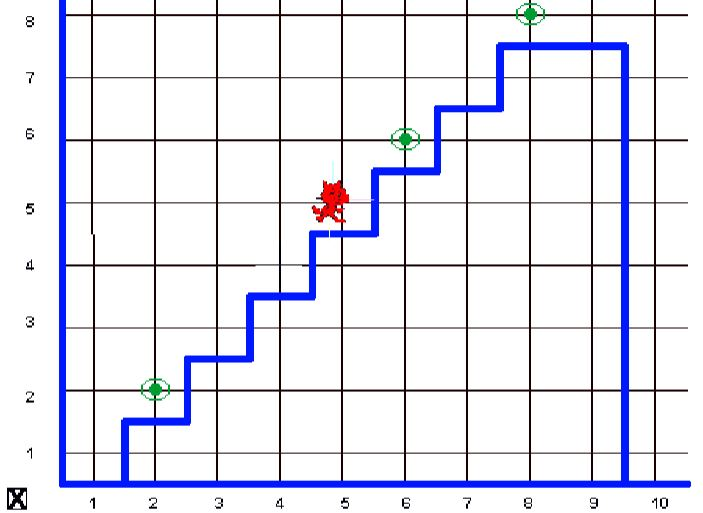
\includegraphics[width=.8\textwidth]{karel}
\end{center}
\caption{Karel the Robot implemented in Scratch; the green dots are the beepers}\label{fig.karel}
\end{figure}

Les communications indirectes combinées à la manipulation peuvent générer des modèles intéressants. La figure \ref{fig.coll1} montre un environnement rempli de petits objets et de cinq robots mobiles équipés de pinces. Les robots suivent un ensemble de règles simples :
\begin{itemize}
\item Si le robot trouve un objet isolé, il le ramasse ;
\item Si le robot trouve un objet isolé mais en tient déjà un, il pose le nouvel objet à côté de celui qui a été trouvé ;
\item Le robot évite les murs et les groupes de plusieurs objets.
\end{itemize}
Il semble que ces règles amènent les robots à placer tous les objets par groupes de deux, mais ce n'est pas le cas, comme le montre la Fig.~\ref{fig.coll2}. La raison en est qu'un groupe d'objets \emph{vus de côté} peut ressembler à un objet isolé, de sorte qu'un objet supplémentaire est placé dans le groupe. Il en résulte que les grands groupes d'objets sont assemblés uniquement par communication indirecte.

\begin{figure}
\begin{minipage}{.45\textwidth}
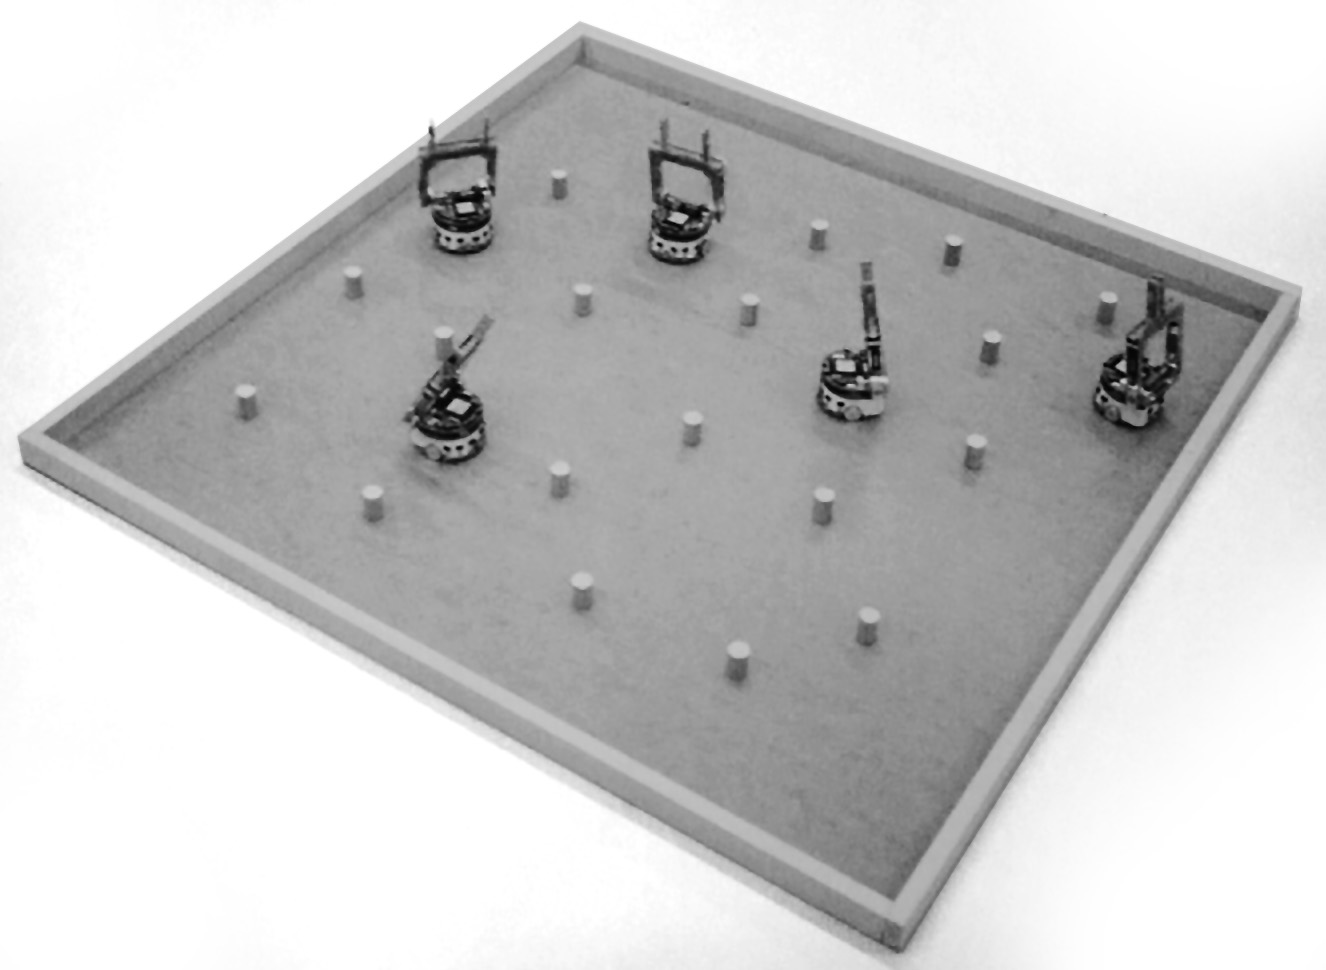
\includegraphics[width=.45\textwidth]{coll1}
\caption{Robots à pince dans un environnement rempli de petits objets}
\label{fig.coll1}
\end{minipage}
\hspace{\fill}
\begin{minipage}{.45\textwidth}
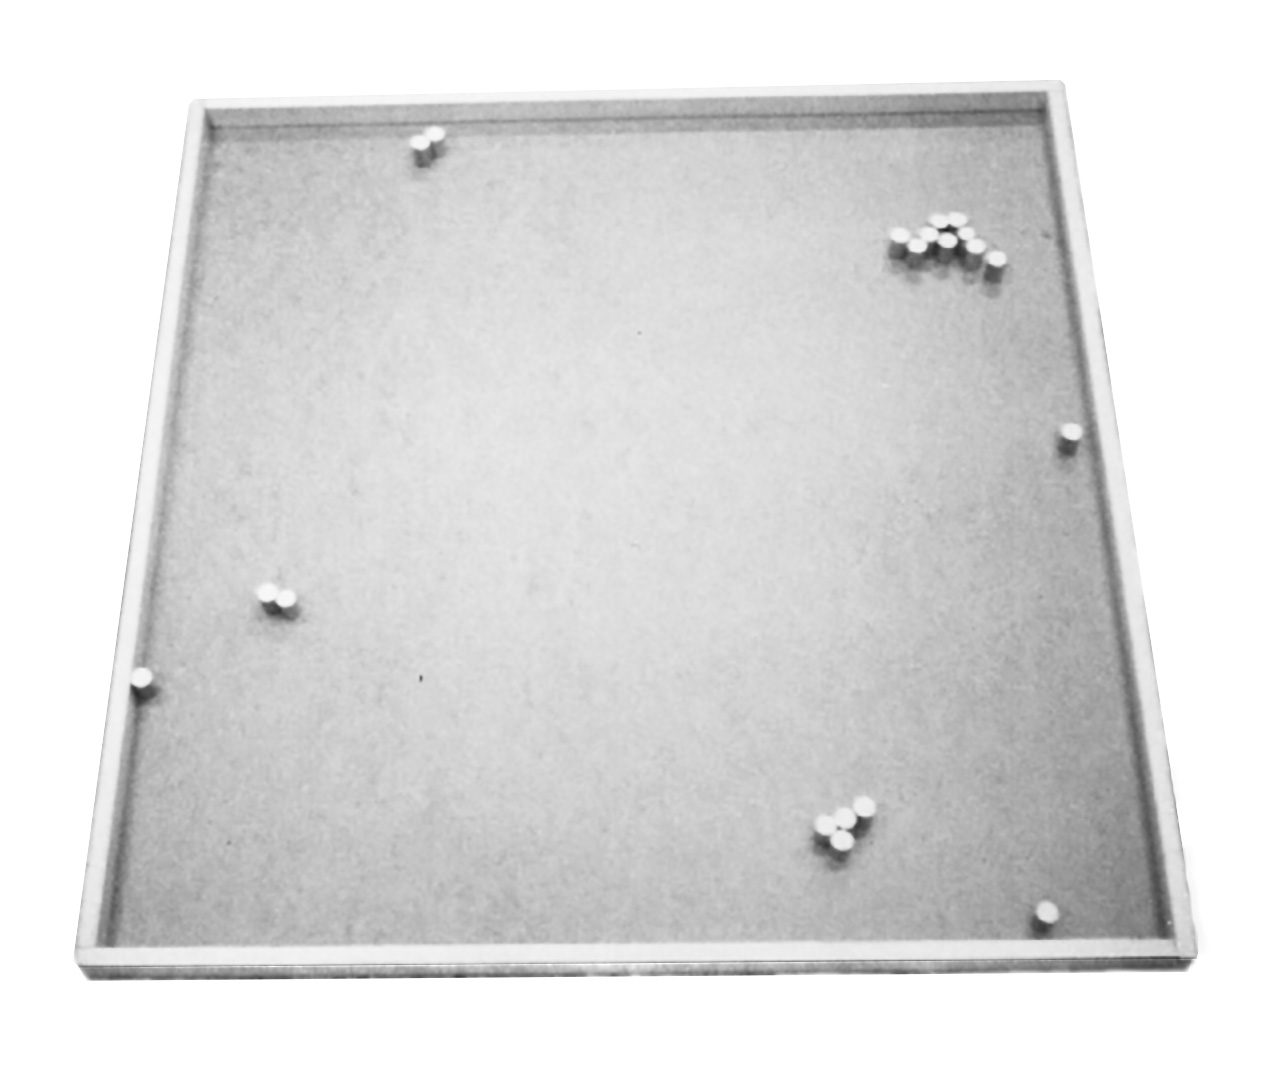
\includegraphics[width=.45\textwidth]{coll2}
\caption{Les objets ont été rassemblés en groupes}
\label{fig.coll2}
\end{minipage}
\end{figure}

\subsection{L'algorithme BeeClust}
\index{robotique en essaim!algorithme BeeClust}

L'algorithme BeeClust est un algorithme d'essaim inspiré du comportement des abeilles. Il utilise une architecture distribuée et des communications locales pour générer un résultat global. L'algorithme BeeClust est basé sur la façon dont les très jeunes abeilles se regroupent autour des endroits où la température est optimale dans l'obscurité de leur nid. Elles mesurent les températures locales et détectent les collisions avec d'autres abeilles.  L'algorithme peut être utilisé par un essaim de robots pour localiser la pollution ; au lieu de mesurer la température, chaque robot mesure une certaine quantité physique qui indique les niveaux de pollution. Avec le temps, les robots se rassembleront en groupes aux endroits où les niveaux de pollution sont élevés.

La figure~\ref{fig.beeclust} montre une machine à états qui met en œuvre l'algorithme. Le robot se déplace au hasard jusqu'à ce qu'il heurte un autre robot. À ce moment-là, il mesure la température à l'endroit de la collision. Il attend à cet endroit pendant une période de temps proportionnelle à la température qu'il a trouvée, puis se remet à se déplacer de manière aléatoire. Lorsque le robot se déplace, il évite les obstacles tels que les murs. L'algorithme utilise ce qui est peut-être la forme la plus simple de communication : la détection d'une collision avec un autre robot. La nature localisée des communications est essentielle au bon fonctionnement de l'algorithme.

\begin{figure}
\begin{center}
\begin{tikzpicture}[node distance = 4cm and 5cm,align=left,minimum size=16mm,every loop/.style={min distance=16mm}]
% Nodes
\node[draw,circle] (moving) {\p{en mouvement}};
\node[draw,circle] (waiting) [right=of moving] {\p{attente}};
% Initial state arrow
\draw[->] (-15mm,10mm) to node [above left,yshift=-3mm] {\p{vrai} $\leadsto$ \p{avant}} (moving);
% Transitions from moving
\path[->] (moving) edge [loop above] node [above,yshift=-4mm] {\p{collision avec un mur} $\leadsto$ \p{tourner au hasard, vers l'avant}} ();
\path[->] (moving) edge node[above] {\p{collision avec le robot} $\leadsto$\\ \p{mesurer la température,}\\\p{calculer le temps d'attente}} (waiting);
% Transitions from waiting
\path[->,bend left=20] (waiting) edge node[below,yshift=3mm] {\p{attente expirée} $\leadsto$ \p{tourner au hasard, vers l'avant}} (moving);
\end{tikzpicture}
\end{center}
\caption{L'algorithme BeeClust}\label{fig.beeclust}
\end{figure}

Au départ, les robots se heurtent à des endroits aléatoires, mais ceux qui se trouvent dans des endroits où la température est plus élevée y restent plus longtemps, ce qui provoque des collisions supplémentaires. À long terme, la plupart des robots formeront un groupe dans la zone où les températures sont les plus élevées. Ils se heurtent fréquemment les uns aux autres, car le fait d'être dans une foule augmente le nombre de collisions. Bien entendu, ce mécanisme ne peut fonctionner qu'avec un grand nombre de robots qui génèrent de nombreuses collisions, ce qui donne lieu à de nombreuses mesures et à la formation de grappes. 

\subsection{L'implémentation ASSISIbf de BeeClust}
\index{robotique en essaim!Mise en œuvre de l'algorithme BeeClust par ASSISIbf}

Dans le cadre du projet ASSISIbf, des chercheurs de l'université de Graz ont utilisé des robots Thymio pour mettre en œuvre l'algorithme BeeClust dans le cadre d'une recherche sur le comportement des abeilles dans un nid. L'algorithme simule un groupe de jeunes abeilles dans une arène circulaire froide, où deux sources de chaleur virtuelles sont placées à droite et à gauche de l'arène. Au départ, une seule de ces sources de chaleur est active. Les sources de chaleur sont simulées par deux groupes de trois robots situés sur les bords de l'arène (Fig.~\ref{fig.beeclust-demo}(a)).

\begin{figure}
\begin{center}
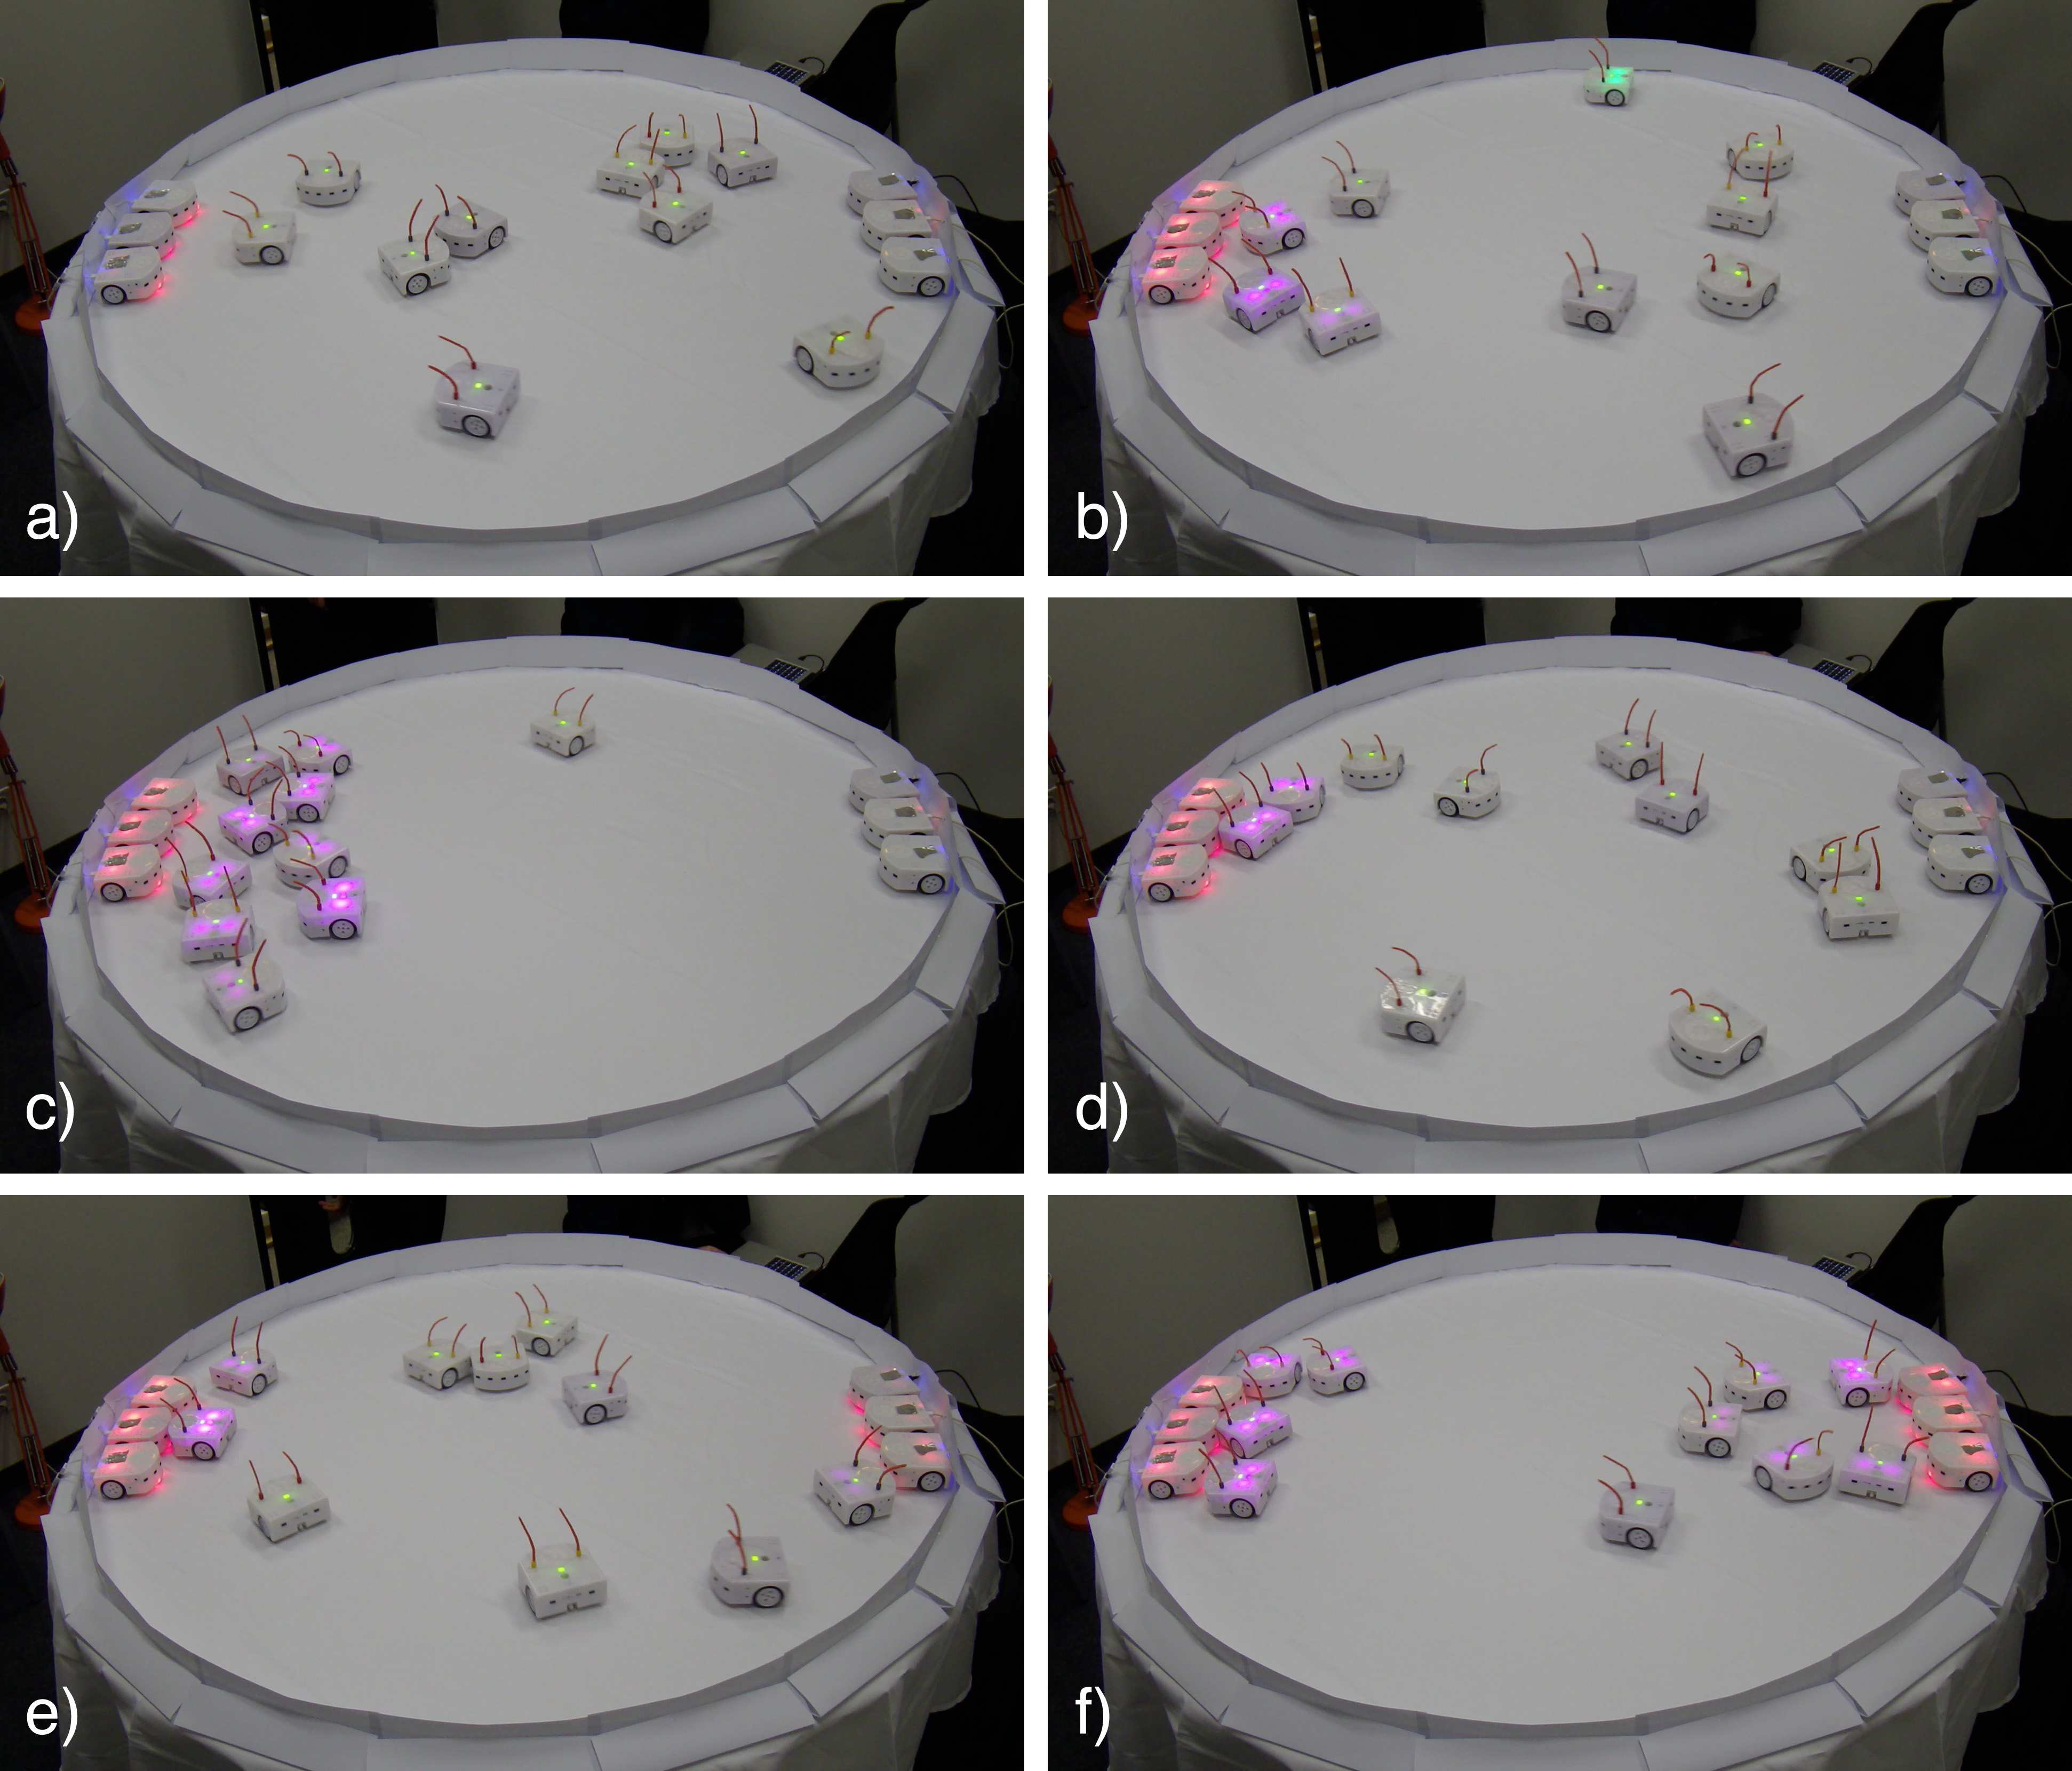
\includegraphics[width=\textwidth]{bee-clust}
\end{center}
\caption{Mise en œuvre de BeeClust. Les photographies ont été prises aux heures suivantes (minutes:secondes) à partir du début de l'expérience : a) 1:40, b) 2:30, c) 9:40, d) 12:40, e) 13:20, f) 21:10.}
\label{fig.beeclust-demo}
\end{figure}

Les trois robots émetteurs de chaleur sur le côté gauche transmettent leur température. Les robots-abeilles qui se trouvent à proximité détectent ce signal et s'arrêtent pendant un temps proportionnel à la température. Pendant leur séjour dans cette zone, ils transmettent également un signal de température. En outre, si les robots émetteurs de chaleur détectent des robots proches, ils augmentent leur chaleur et transmettent la nouvelle température. La figure \ref{fig.beeclust-demo} montre l'évolution du comportement des robots : (a) l'état initial lorsque les robots commencent à se déplacer et que seule la source de température de gauche est allumée ; (b) les robots commencent à se regrouper autour de la source de gauche ; (c) le niveau de regroupement le plus élevé se produit. Les robots-abeilles peuvent quitter la grappe, explorer l'environnement et revenir à la grappe, comme le montre la figure (d). Ce phénomène est dû à la nature aléatoire de l'algorithme et est essentiel pour éviter que le système ne soit piégé dans des minima locaux. La figure \ref{fig.beeclust-demo}~(e) montre le moment où la bonne source est également activée. Après environ $21$ minutes, les robots forment deux groupes plus petits (f).

\begin{framed}
\act{algorithme BeeClust}{beeclust-swarm-act}
\begin{itemize}
\item Mettre en œuvre l'algorithme BeeClust pour amener un groupe de robots à se regrouper à l'endroit le plus lumineux d'une pièce.
\item Utiliser trois capteurs : un capteur de lumière pour mesurer la lumière ambiante, un capteur pour détecter les autres robots et un capteur pour détecter les limites de l'arène.
\item Solution 1 : Utiliser des capteurs de proximité pour détecter les autres robots et des capteurs au sol pour détecter une ligne définissant les limites de l'arène.
\item Solution 2 : Définissez les limites de l'arène à l'aide d'un mur et utilisez les communications entre robots pour faire la distinction entre les robots et le mur. Pour éviter toute confusion, n'utilisez pas le même capteur pour détecter les autres robots et le mur.
\end{itemize}
\end{framed}

\section[Robot basée sur les interactions physiques]{Robotique en essaim basée sur les interactions physiques}\label{s.swarm-physical}

Dans la Sect.~\ref{s.no-localization}, nous avons étudié un exemple typique de comportement efficace en essaim : une colonie de fourmis trouvant un chemin entre leur nid et une source de nourriture. Cet exemple utilisait des communications indirectes sous la forme de phéromones déposées sur le sol. Dans cette section, nous examinons une autre forme de comportement en essaim qui est médiée par des interactions physiques. Nous commençons par des fourmis collaborant à l'extraction d'un bâton du sol et à une version robotisée de cette tâche. Nous examinerons ensuite la manière dont les forces exercées par plusieurs robots peuvent être combinées, comme le montre un algorithme simple mais astucieux appelé "poussée collective basée sur l'occlusion".

\subsection{Collaboration à une tâche physique}
\index{robotique en essaim!collaboration physique}

La figure~\ref{fig.real-ants-pulling} montre deux fourmis extrayant un bâton du sol pour l'utiliser dans la construction d'un nid. Le bâton est enfoncé si profondément qu'une fourmi ne peut pas l'extraire seule. Nous voulons concevoir un système robotique pour accomplir cette tâche (Fig.~\ref{fig.robots-pulling}). Chaque robot cherche au hasard jusqu'à ce qu'il trouve un bâton. Il tire alors sur le bâton aussi fort que possible. S'il réussit à extraire le bâton, il le ramène dans un nid ; sinon, comme il n'a que partiellement extrait le bâton, il attend de sentir qu'un autre robot tire plus fort et relâche le bâton. Si aucun robot ne lui vient en aide pendant un certain temps, le robot relâche sa prise et retourne à une recherche aléatoire. Ainsi, s'il y a plus de bâtons que de robots, le système ne se bloquera pas, chaque robot essayant d'extraire un bâton et attendant indéfiniment.

\begin{figure}
\begin{minipage}{.45\textwidth}
\includegraphics[width=.45\textwidth]{real-ants-pulling}
\caption{Ants tirant un bâton du sol}
\label{fig.real-ants-pulling}
\end{minipage}
\hspace{\fill}
\begin{minipage}{.45\textwidth}
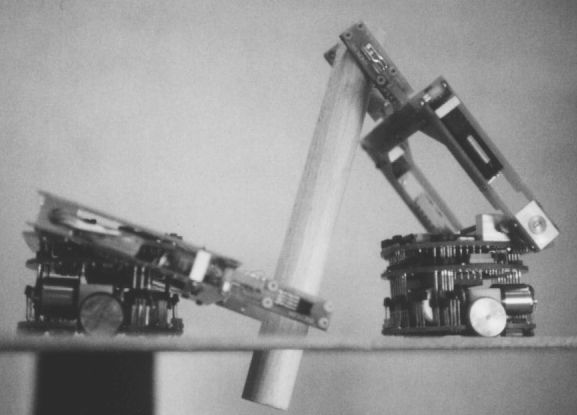
\includegraphics[width=.45\textwidth]{robots-pulling}
\caption{Les robots tirent un bâton du sol}
\label{fig.robots-pulling}
\end{minipage}
\end{figure}

La machine à états finis de cet algorithme est présentée dans la Fig.~\ref{fig.antspulling-FSM}. Bien que ce comportement soit simple et local, lorsqu'il est appliqué par deux robots, il permet d'extraire le bâton du sol. Le robot de droite sur la Fig.~\ref{fig.robots-pulling} tire une partie du bâton aussi loin que possible du sol en utilisant le mouvement maximal de son bras. Lorsqu'il détecte qu'un autre robot a trouvé le même bâton et commence à tirer, le premier robot relâche le bâton pour permettre au second robot de l'extraire. En combinant les capacités physiques de deux robots avec une simple spécification de comportement, nous obtenons un résultat qu'aucun des robots ne pourrait atteindre seul.

\begin{figure}
\begin{center}
\begin{tikzpicture}[node distance = 2.5cm and 40mm,align=left,minimum size=14mm,every loop/.style={min distance=16mm}]
% Nodes
\node[draw,circle] (looking) {\p{recherche}};
\node[draw,circle] (lifting) [right=of looking] {\p{levage}};
\node[draw,circle] (to-home) [below=of lifting] {\p{amener}\\\p{ au nid}};
\node[draw,circle] (waiting) [below=of looking] {\p{attente}};
% Initial state arrow
\draw[->] (-10mm,10mm) to node [above,yshift=0mm] {\p{vrai} $\leadsto$\\\p{avant, régler le délai de recherche}} (looking);
% Transitions from searching
\path[->] (looking) edge [loop left] node [below,yshift=-2mm] {\p{délai de recherche} $\leadsto$\\\p{tourner au hasard,}\\\p{avant}} ();
\path[->] (looking) edge node[above,xshift=-2mm,yshift=-5mm] {\p{trouvé} $\leadsto$  \p{saisir et soulever}} (lifting);
% Transitions from lifting
\path[->] (lifting) edge node[right] {\p{extrait} $\leadsto$\\ \p{aller au nid}} (to-home);
\path[->,bend left=10] (lifting) edge node[above,yshift=6mm,xshift=3mm] {\p{levage maximal atteint,}\\\p{non extrait} $\leadsto$\\\p{define the waiting time}} (waiting);
% Transitions from to nest
\path[->,bend left=10] (to-home) edge node[left,yshift=-12mm,xshift=20mm] {\p{au nid} $\leadsto$} (looking);
% Transitions from waiting
\path[->,bend right=20] (waiting) edge node[right] {\p{attendre}\\\p{délai d'attente} $\leadsto$} (looking);
\path[->,bend left=20] (waiting) edge node[left,yshift=-8pt] {\p{un autre robot}\\\p{tirant} $\leadsto$ \\\p{relâcher le bâton}} (looking);
\end{tikzpicture}
\end{center}
\caption{Algorithme pour le tirage distribué de bâtons}\label{fig.antspulling-FSM}
\end{figure}

\subsection{Combiner les forces de plusieurs robots}
\index{robotique en essaim!combiner les forces}

\ref{fig.pulling1} montre un robot à entraînement différentiel se déplaçant à reculons (de gauche à droite). Il exerce une force $F_r$ qui peut être utilisée pour tirer un objet. La figure~\ref{fig.pulling2} montre deux robots connectés ensemble de sorte qu'ils exercent une force $F_{sub{total}}$ lorsqu'ils se déplacent de gauche à droite.

\begin{figure}
\begin{center}
\begin{tikzpicture}
\pic[scale=.7] at (0,0) { robot-side };
\draw[->,thick] (-1.6,.7) -- node[above left] {$F_r$} (1,.7);
\end{tikzpicture}
\caption{Un robot qui tire avec une force donnée $F_r$}\label{fig.pulling1}
\end{center}
\end{figure}

\begin{figure}
\begin{center}
\begin{tikzpicture}[scale=.6]
\pic[rotate=-20,scale=.7] at (0,0) { robot-side };
\pic[rotate=-20,scale=.7] at (8.5,-.4) { robot-side };
\draw[->,thick] (-1.3,0.8) -- node[above left] {$F_{\textit{total}}$} (1,0.8);
\draw[fill,gray!60] (62mm,2mm) -- ++(70:7mm) -- ++(-20:10mm) -- ++(70:25mm) -- ++(-20:25mm) -- ++(-110:6.3mm) -- ++(160:19mm) -- ++(-110:26mm) -- cycle;
\path (13,-3) rectangle ++(1,-3mm);  % Dummy for extra space
\end{tikzpicture}
\caption{Deux robots connectés se tirent avec une force donnée $F_{total}$}\label{fig.pulling2}
\end{center}
\end{figure}

Quelle est la relation entre $F_r$ et $F_{\sub{total}}$ ? Il y a trois possibilités :
\begin{itemize}
\item $F_{\sub{total}} < 2 F_r$ : Les robots connectés perdent en efficacité car la force qu'ils exercent est inférieure à celle exercée par les deux robots tirant séparément.
\item $F_{\sub{total}} = 2 F_r$ : Les robots connectés ont la même efficacité que deux robots séparés.
\item $F_{\sub{total}} = 2 F_r$ : Les robots connectés atteignent la même efficacité que deux robots séparés.
\end{itemize}
Les robots peuvent atteindre $F_{\sub{total}} > 2 F_r$, où la force totale est supérieure à la somme des forces exercées par les robots individuels, car dans certaines configurations mécaniques, les robots connectés sont plus stables car leur centre de gravité est mieux placé. 

\begin{framed}
\act{Force de traction de plusieurs robots.}{pulling_force}
\begin{itemize}
\item Connectez deux robots et vérifiez s'ils exercent une force inférieure, égale ou supérieure au double de celle exercée par un seul robot. Vous pouvez relier les robots à l'aide d'une connexion rigide comme sur la Fig.~\ref{fig.pulling2} ou à l'aide d'une connexion flexible en utilisant une ficelle.
\item Mesurer $F_r$, la force exercée par un seul robot, puis mesurer $F_{sub{total}}$ la force exercée par les robots connectés.
\item Un \emph{dynamomètre} (Fig~\ref{fig.dyna}) est le meilleur instrument pour mesurer les forces. Si vous n'en disposez pas, vous pouvez utiliser un câble, une poulie et des poids (ou une balance) comme indiqué sur la Fig.~\ref{fig.scale}.
\item Changez l'orientation des robots : tirez vers l'avant au lieu de tirer vers l'arrière. Cela change-t-il le résultat ?
\item Faire des expériences sur différentes surfaces (sol dur, moquette, papier) et déterminer l'effet de la surface sur la force résultante.
\end{itemize}
\end{framed}

\begin{figure}
\begin{center}
\begin{tikzpicture}[scale=.8]
% Table
\draw[fill,gray] (-6,-7.2mm) rectangle +(12,2mm);
\draw[fill,gray] (-5,-7.2mm) rectangle +(4mm,-4mm);
\draw[fill,gray] (5,-7.2mm) rectangle +(4mm,-4mm);
% Robot
\pic[scale=.6] at (0,0) { robot-side };
\draw[->,thick] (3.7,.7) -- node[above] {$F_r$} (6,.7);
% Attachment
\draw (-3,8mm) rectangle +(2,4mm);
\draw (-1,1) -- (0,1);
% Spring
\draw (-20mm,14mm) -- (-50mm,14mm) -- (-50mm,6mm) -- (-20mm,6mm);
\draw (-50mm,10mm) -- (-60mm,10mm);
\draw (-50mm,10mm) -- ++(2mm,2mm) -- ++(2mm,-4mm) -- ++(2mm,4mm)  -- ++(2mm,-4mm) -- ++(2mm,4mm)  -- ++(2mm,-4mm) -- ++(2mm,4mm)  -- ++(2mm,-4mm) -- ++(2mm,4mm)  -- ++(2mm,-3mm);
\end{tikzpicture}
\caption{Mesure de la force à l'aide d'un dynamomètre}\label{fig.dyna}
\end{center}
\end{figure}

\begin{figure}
\begin{center}
\begin{tikzpicture}
% Table
\draw[fill,gray] (-2,-9mm) rectangle +(8,2mm);
\draw[fill,gray] (-1,-9mm) rectangle +(4mm,-15mm);
\draw[fill,gray] (5,-9mm) rectangle +(4mm,-15mm);
% Robot
\pic[scale=.6] at (0,-2.7mm) { robot-side };
\draw[->,thick] (3,.3) -- node[above] {$F_r$} (6,.3);
% Attachment
\draw[fill,gray!80] (-3,1mm) circle[radius=3mm];
\draw (-2.9,1mm) -- (-3.1,1mm);
\draw (-3,0mm) -- (-3,2mm);
\draw (-3,.4) -- (0,.4);
\draw (-33mm,2mm) -- ++(0,-19mm);
\draw[fill,gray!80] (-35mm,-16mm) rectangle +(4mm,4mm);
\draw (-40mm,-24mm) rectangle +(14mm,8mm);
\draw (-33mm,-20mm) circle[radius=3mm];
\draw[->] (-33mm,-20mm) -- +(30:3mm);
\end{tikzpicture}
\caption{Mesure de la force à l'aide d'un poids et d'une balance}\label{fig.scale}
\end{center}
\end{figure}

\subsection{poussée collective basée sur l'occlusion}
\index{robotique en essaim!poussée collective basée sur l'occlusion}

Considérons un autre exemple de combinaison de la force de plusieurs robots. Au lieu d'un lien physique comme dans la Fig.~\ref{fig.pulling2}, nous utilisons de nombreux robots simples pour pousser un objet, imitant un groupe de fourmis. Une fois encore, les avantages d'un système distribué sont la flexibilité - l'engagement des seules ressources nécessaires à la tâche - et la robustesse - si un robot tombe en panne, l'objet peut se déplacer un peu plus lentement, mais il n'y a pas d'échec total de la tâche. Ces avantages s'accompagnent de ressources supplémentaires et de la complexité de la mise en œuvre de la coordination entre les robots.

La figure \ref{fig.swarm-pushing} montre un groupe de petits robots poussant un grand objet représenté par un cercle vers un objectif. Une approche consisterait à déterminer la direction de l'objectif, à partager cette information entre tous les robots et à demander à chaque robot de calculer la direction dans laquelle il doit pousser. Ce n'est pas aussi simple qu'il n'y paraît, car un simple robot peut ne pas être en mesure de déterminer sa position et son cap absolus.

Une approche de robotique en essaim est appelée \emph{poussée basée sur l'occlusion}, qui suppose que les robots n'ont qu'une connaissance locale, et non globale, de ce que font les autres robots. Les robots sont en mesure de déterminer s'ils peuvent ou non détecter l'objectif. Par exemple, une lumière vive peut être installée sur l'objectif et les robots équipés d'un capteur de lumière. 

\begin{figure}
\begin{center}
\begin{tikzpicture}[scale=1.1]
\node[circle,draw,thick] (center) at (0,0) [minimum size=40mm] {};
\coordinate (goal) at (6,1.5);
\draw[fill] (goal) circle [radius=1pt];
\draw[->,shorten >= 50mm] (0,0) -- (goal);
\node at (6.5,1.5) {\p{goal}};
% Use negative shorten arrow trick to extend the tangent lines
\draw[shorten >= -50mm] (goal) -- (tangent cs:node=center, point={(goal)}, solution=1);
\draw[shorten >= -50mm] (goal) -- (tangent cs:node=center, point={(goal)}, solution=2);
% Draw the pushing robots
\foreach \angle/\x/\y in { 0/0mm/0mm, -20/2mm/10mm, -40/7mm/18mm, 20/2mm/-10mm, 40/7mm/-18mm, 60/14mm/-22mm } {
  \pic[rotate=\angle,scale=0.3] at (\x-24mm, \y) { robot };
  \draw[->] (\x-24mm,\y) -- +(\angle:8mm);
}
% Draw the non-pushing robots
\pic[rotate=-80,scale=0.3] at (0mm, 28mm) { robot };
\path[->,bend right=40,red,thick] (0mm,28mm) edge (8mm,26mm);
\pic[rotate=60,scale=0.3] at (8mm, -28mm) { robot };
\path[->,bend left=30,red,thick] (8mm,-28mm) edge (16mm,-24mm);
\pic[rotate=-120,scale=0.3] at (30mm, 10mm) { robot };
\path[->,bend right=50,red,thick] (30mm,10mm) edge (36mm,4mm);
\end{tikzpicture}
\end{center}
\caption{Coordination basée sur l'occlusion : flèches noires droites pour les robots qui poussent l'objet et flèches rouges courbes pour les robots qui recherchent une position occluse.}\label{fig.swarm-pushing}
\end{figure}

Figure~\ref{fig.FSM-swarm-pushing} shows the finite state machine for this algorithm. The robots search for the object; when they find it they place themselves perpendicular to the surface and push (straight black arrows). This could be implemented using a touch sensor or a proximity sensor. The robots continue to push as long as they \emph{do not} detect the goal. If they do detect the goal, they stop pushing, move away (curved red arrows) and commence a new search for an occluded position where they resume pushing. The result is that the vector sum of the forces exerted by the robots is in a direction that moves the object toward the goal. The occlusion algorithm leads to the task being performed without a central control unit and even without inter-robot communications.

\begin{figure}
\begin{center}
\begin{tikzpicture}[node distance = 4cm and 4cm,align=left,minimum size=16mm,every loop/.style={min distance=16mm}]
% Nodes
\node[draw,circle] (searching) {\p{recherche}\\\p{pour l'objet}}; and their fit to the required performances of the system.
\node[draw,circle] (pushing) [right=of searching] {\p{poussant}};
% Initial state arrow
\draw[->] (-5mm,12mm) to node [above left,yshift=-2mm,xshift=6mm] {\p{vrai} $\leadsto$\\\p{se déplacer au hasard}} (searching);
% Transitions from searching
\path[->,bend left=30] (searching) edge node [above,yshift=-4mm] {\p{objet trouvé et but occulté} $\leadsto$\\\p{pousser l'objet}} (pushing);
% Transitions from pushing
\path[->] (pushing) edge [loop right] node[below,xshift=-5mm,yshift=-3mm] {\p{but occulté} $\leadsto$} (pushing);
\path[->,bend left=30] (pushing) edge node[below,yshift=4mm] {\p{objectif visible} $\leadsto$\p{se déplacer au hasard}} (searching);
\path[->] (pushing) edge node[above,yshift=-6mm] {\p{objet perdu} $\leadsto$\p{se déplacer au hasard}} (searching);
\end{tikzpicture}
\end{center}
\caption{Algorithme pour la coordination basée sur l'occlusion}\label{fig.FSM-swarm-pushing}
\end{figure}

\begin{framed}
\act{Force totale}{Force totale}
\begin{itemize}
\item Considérons la configuration montrée sur la Fig.~\ref{fig.total-force}. Le robot $1$ pousse un objet à un angle de $45^{\circ}$ avec la force $f_1$, le robot $2$ pousse horizontalement avec la force $f_2$ et le robot $3$ pousse verticalement avec la force $f_3$. Montrer que $f_{\sub{total}}$, la force totale sur l'objet, a une magnitude :
\[
\sqrt{\left(f_2+\frac{f_1}{\sqrt{2}}\right)^2+\left(f_3-\frac{f_1}{\sqrt{2}}\right)^2}\,.
\]
dans la direction :
\[
\alpha = \tan^{-1} \frac{2f_3-\sqrt{2}f_1}{2f_2+\sqrt{2}f_1}\,.
\]
\item Calculer l'amplitude et la direction de $f_{\sub{total}}$ pour différentes valeurs des forces individuelles. Si $f_1=f_2=f_3=1$, la magnitude est $\sqrt{3}$ et la direction est $9.7^{\circ}$. Si $f_1=f_2=1$, quelle doit être la valeur de $f_3$ pour que $\alpha=45^{\circ}$ ?
\item Utilisez trois robots pour mettre en oeuvre cette configuration et vérifiez que l'objet se déplace dans la direction calculée.
\end{itemize}
\end{framed}

\begin{figure}
\begin{center}
\begin{tikzpicture}[scale=1.2]
\draw[fill] (0,0) circle [radius=4pt];
\draw[->] (-3,0) -- node[above,near start] {$f_2$} (-4pt,0);
\draw[->] (0,-2) -- node[left,near start] {$f_3$} (0,-4pt);
\draw[->] (-45:-3) -- node[above,near start,yshift=4pt] {$f_1$} (-2pt,2pt);
\draw (-10mm,0) arc (180:135:10mm) node[midway,xshift=-3mm,yshift=1mm] {$45^{\circ}$};
\draw[dashed] (0,0) -- (3,0);
\draw[->] (0,0) -- node[above,near end,xshift=-1mm] {$f_{\sub{total}}$} (20:3);
\draw (15mm,0) arc (0:20:15mm) node[right,midway] {$\alpha$};
\end{tikzpicture}
\caption{La force totale de trois robots}\label{fig.total-force}
\end{center}
\end{figure}

\begin{framed}
\act{poussée basée sur l'occlusion}{occulsion-swarm}
\begin{itemize}
\item Placez trois robots autour d'un objet et placez un objectif à une certaine distance du robot. Mettez en place un mécanisme permettant aux robots de déterminer la direction vers le but, par exemple en attachant une lumière au but ou en plaçant le but au point le plus bas d'une surface inclinée.
\item Mettre en œuvre un mécanisme permettant aux robots de faire la distinction entre l'objet et la limite de la surface sur laquelle ils se déplacent. Par exemple, utiliser un ruban noir sur la surface comme limite et détecter l'objet à l'aide de capteurs de proximité.
\item Mettre en place un mécanisme pour que les robots ne se poussent pas les uns les autres. Une méthode consisterait à utiliser un capteur de couleur et à attacher du ruban adhésif de couleur aux robots.
\item Mettre en œuvre l'algorithme de poussée basé sur l'occlusion.
\item Discuter de la possibilité d'utiliser la poussée basée sur l'occlusion en trois dimensions, par exemple, des robots sous-marins poussant un objet.
\end{itemize}
\end{framed}

\section{Résumé}

La robotique en essaim utilise plusieurs robots dans une architecture distribuée pour effectuer une tâche. Avec une architecture distribuée, le système est résistant aux défaillances des robots individuels et flexible dans sa capacité à ajouter ou supprimer des robots lorsque l'échelle de la tâche change. Une architecture distribuée peut effectuer des tâches que les robots individuels ne peuvent pas réaliser, comme nous l'avons vu dans les exemples de robots combinant leurs forces. Enfin, plusieurs robots peuvent agir simultanément à différents endroits éloignés les uns des autres. Ces avantages ont un prix : l'augmentation du coût des robots multiples, la complexité des mécanismes de coordination à mettre en œuvre et, dans certains cas, la perte de performance due au chevauchement entre les actions des différents robots. 


\section{Lecture complémentaire}

Un aperçu de la robotique collective est donné dans \cite{kernbach2013handbook} et la collection~\cite{sahin2005} se concentre sur la robotique en essaim. Pour les projets spécifiques présentés dans ce chapitre, voir :
\begin{itemize}
\item Karel le robot~\cite{karel}.
\item BeeClust~\cite{bodi2012interaction} et~\cite{Schmickl2009}.
\item ASSISIbf~\cite{schmickl2013assisi} et \url{http://assisi-project.eu}.
\item Interaction physique (tirer un bâton)~\cite{Ijspeert2001}.
\item Transport basé sur l'occlusion~\cite{chen2013strategy} et \cite{gross2015}.
\end{itemize}

